\documentclass[12pt, twoside]{article}
\usepackage[francais]{babel}
\usepackage[T1]{fontenc}
\usepackage[latin1]{inputenc}
\usepackage[left=7mm, right=7mm, top=7mm, bottom=7mm]{geometry}
\usepackage{float}
\usepackage{graphicx}
\usepackage{array}
\usepackage{multirow}
\usepackage{amsmath,amssymb,mathrsfs} 
\usepackage{soul}
\usepackage{textcomp}
\usepackage{eurosym}
\usepackage{lscape}
 \usepackage{variations}
\usepackage{tabvar}
 
\pagestyle{empty}

\title{\ul{\textbf{Proportionnalit� des longueurs d'un triangle}}}
\date{}

\begin{document}
\maketitle

\fbox{
\begin{minipage}{18cm}
\ul{Propri�t�}: Si dans un triangle ABC, M est un point de [AB], N un point de
[AC] et (MN) est parall�le � (BC) alors: 

\begin{center}
$\dfrac{AM}{AB}=\dfrac{AN}{AC}=\dfrac{MN}{BC}$.
\end{center}
\end{minipage}
}

\bigskip

\ul{Exemple}:  

\enskip

\begin{tabular}{cc}
\begin{minipage}{9cm}
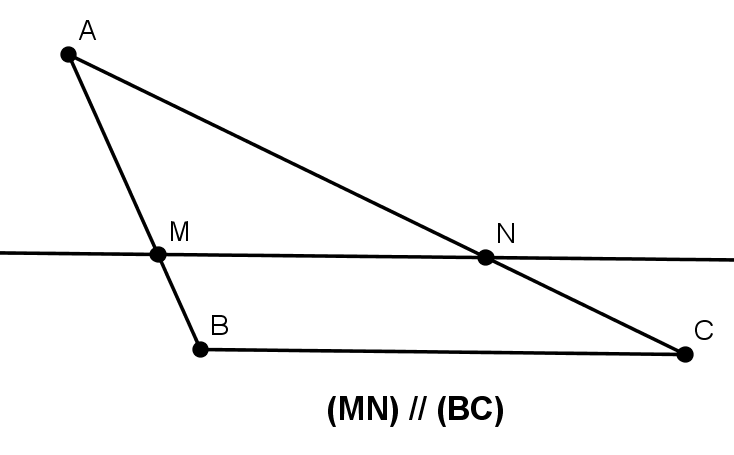
\includegraphics[width=6cm]{images/ex1.png}
\end{minipage}
&
\begin{minipage}{9cm}
Alors: $\dfrac{AM}{AB}=\dfrac{AN}{AC}=\dfrac{MN}{BC}$
\end{minipage}
\end{tabular}


\medskip

\ul{M�thode pour calculer une longueur}:

\begin{tabular}{cc}
\begin{minipage}{10cm}
Sur la figure ci-contre, les droites (OL) et (TE) sont parall�les. On donne
HE=5cm, HL=2cm, TE=7cm et HO=3cm. Calculer les longueurs HT et OL.

\end{minipage}
&
\begin{minipage}{8cm}
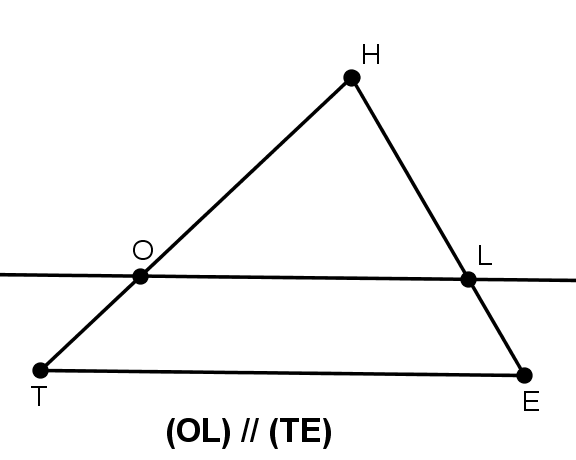
\includegraphics[width=5cm]{images/ex2.png}
\end{minipage}
\end{tabular}


\bigskip



 Dans le triangle THE, on sait que:

\begin{itemize}
  \item [$\bullet$] O $\in$ [HT]
  \item [$\bullet$] L $\in$ [HE]
  \item [$\bullet$] (OL)//(TE). 
  
\end{itemize}

D'apr�s la propri�t� de proportionnalit� des longueurs dans un triangle, on a:
$\dfrac{HO}{HT}=\dfrac{HL}{HE}=\dfrac{OL}{TE}$.

En rempla�ant par les valeurs num�riques:
$\dfrac{3}{HT}=\dfrac{2}{5}=\dfrac{OL}{7}$


\enskip

\textbf{Calcul de HT:} $\dfrac{3}{HT}=\dfrac{2}{5}$ donc $2 \times HT= 3 \times
5$ d'o� $HT= \dfrac{3 \times 5}{2}=7,5$cm.

\enskip

\textbf{Calcul de OL:} $\dfrac{OL}{7}=\dfrac{2}{5}$ donc $2
5 \times OL= 2 \times 7$ d'o� $OL= \dfrac{2 \times 7}{5}=2,8$cm.


\end{document}
